\chapter{Beispielapp}\label{chap:example}
%
Während der Entwicklung wurde ein Beispielapp geschrieben, mit dem auch die Implementierung getestet wurde. Wenn dieses gestartet wird, sieht man das in \autoref{fig:ex} dargestellte UI. Clientseite und Serverseite wurden zur Einfachheit halber in einem App geschrieben. Durch drücken des jeweiligen Buttons kann entschieden werden, welche Seite das Gerät übernehmen soll.
\begin{figure}[htbp]
  \centering
  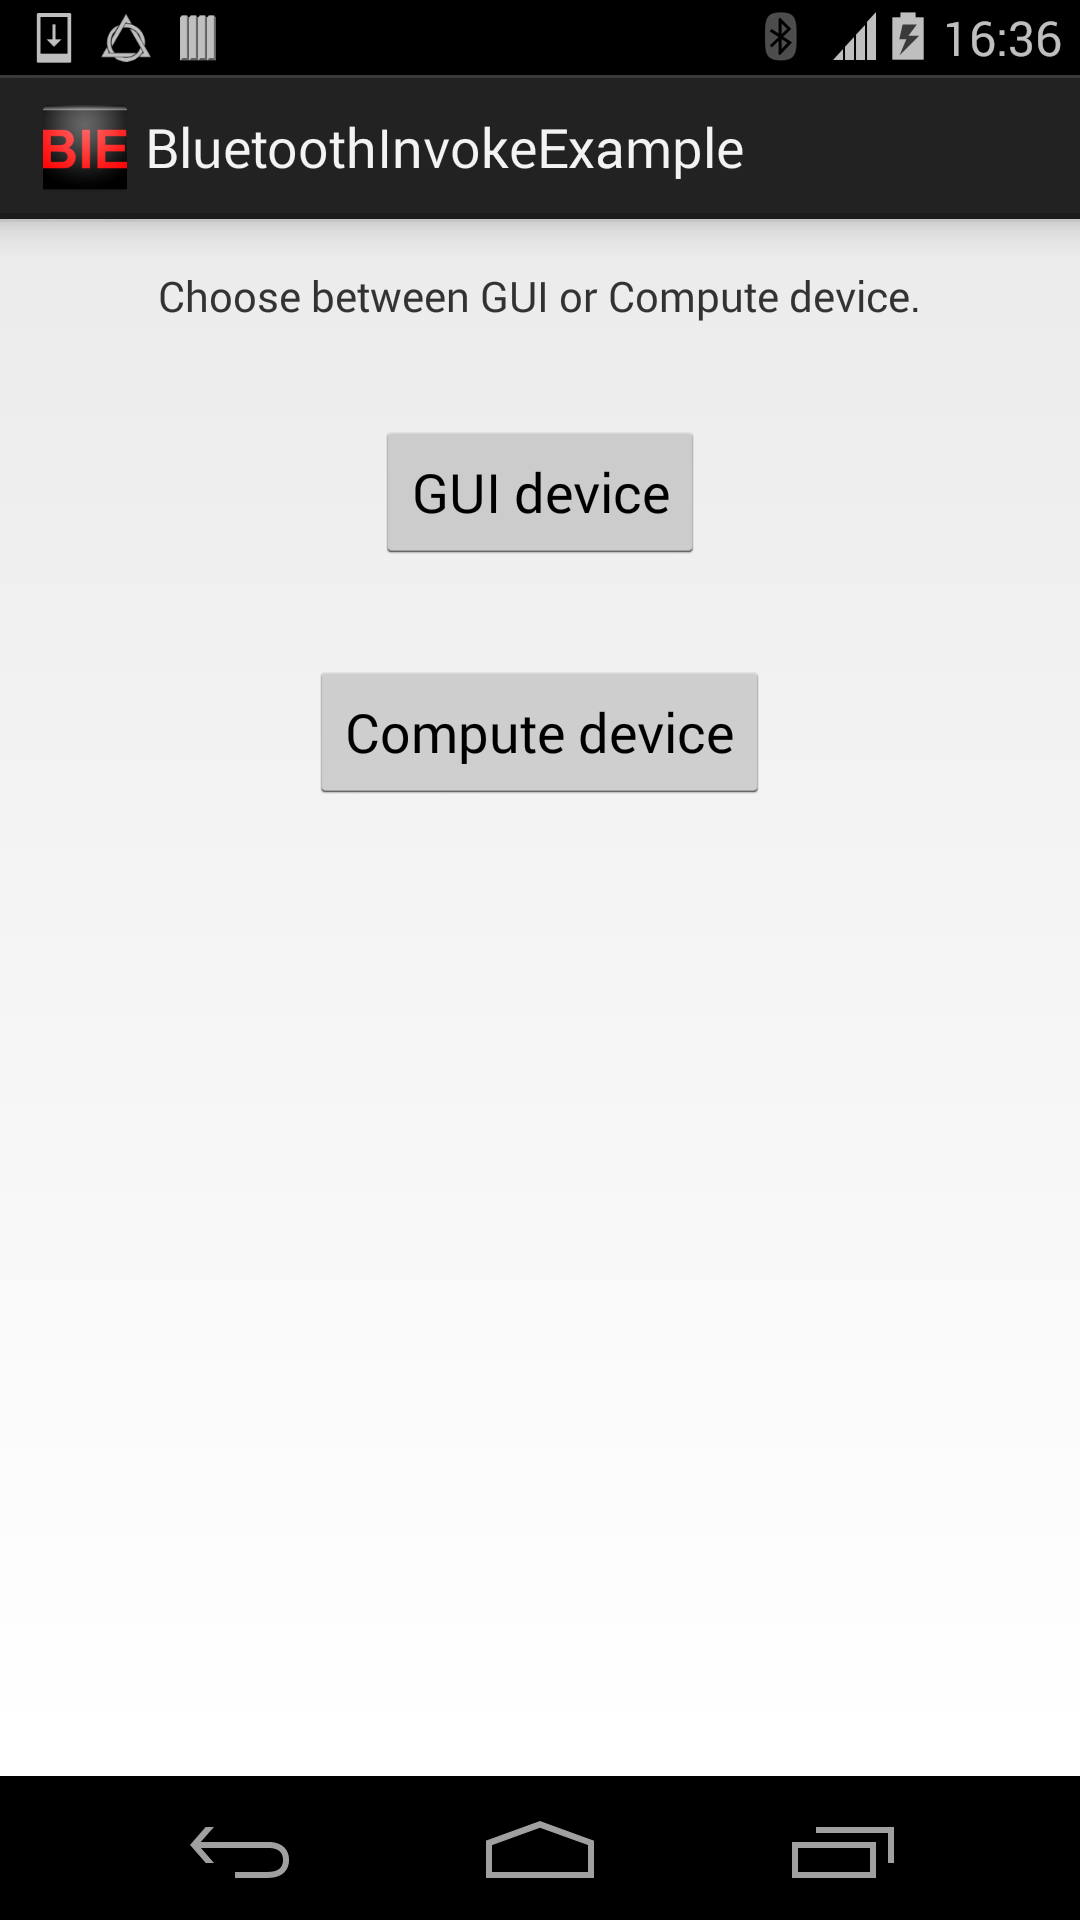
\includegraphics[width=.4\textwidth,keepaspectratio]{ex}
  \caption{UI von \lstinline{ComputeActivity}}
  \label{fig:ex}
\end{figure}

Die Activity der Serverseite hat die in \autoref{fig:ex_ui} gezeigte Oberfläche. Im oberen Teil des Bildschirmes werden Statusnachrichten angezeigt, die von der Bluetooth Verbindung und den Services verschickt werden. Im unteren Teil sind drei Buttons welche jeweils ein Methodenaufruf über Bluetooth verursachen. Die ersten beiden arbeiten direkt mit dem BroadcastReciever in der Activity während der dritte Knopf die Proxy Variante benutzt. Der Aufruf findet dank \emph{Android Annotations} in einem Hintergrund Thread statt.

\autoref{fig:ex_compute} zeigt die Oberfläche auf der Clientseite. Hier zeigt der obere Teil ebenfalls Statusmeldungen. Der \emph{Connect} Button. Sendet ein Intent mit \lstinline{ACTION_CONNECT} zum \lstinline{BTInvokeClientService}. Dies muss geschehen bevor auf der Serverseite die Beispiele ausgeführt werden können.
%

\begin{minipage}{.5\textwidth}
    \centering
    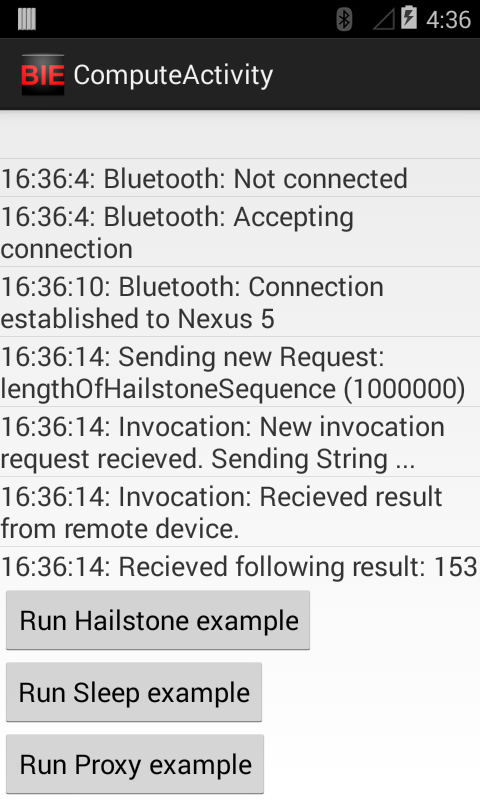
\includegraphics[width=.8\textwidth,keepaspectratio]{ex_ui}
    \captionof{figure}{UI von \lstinline{GUIActivity}}
    \label{fig:ex_ui}
\end{minipage}
\begin{minipage}{.5\textwidth}
    \centering
    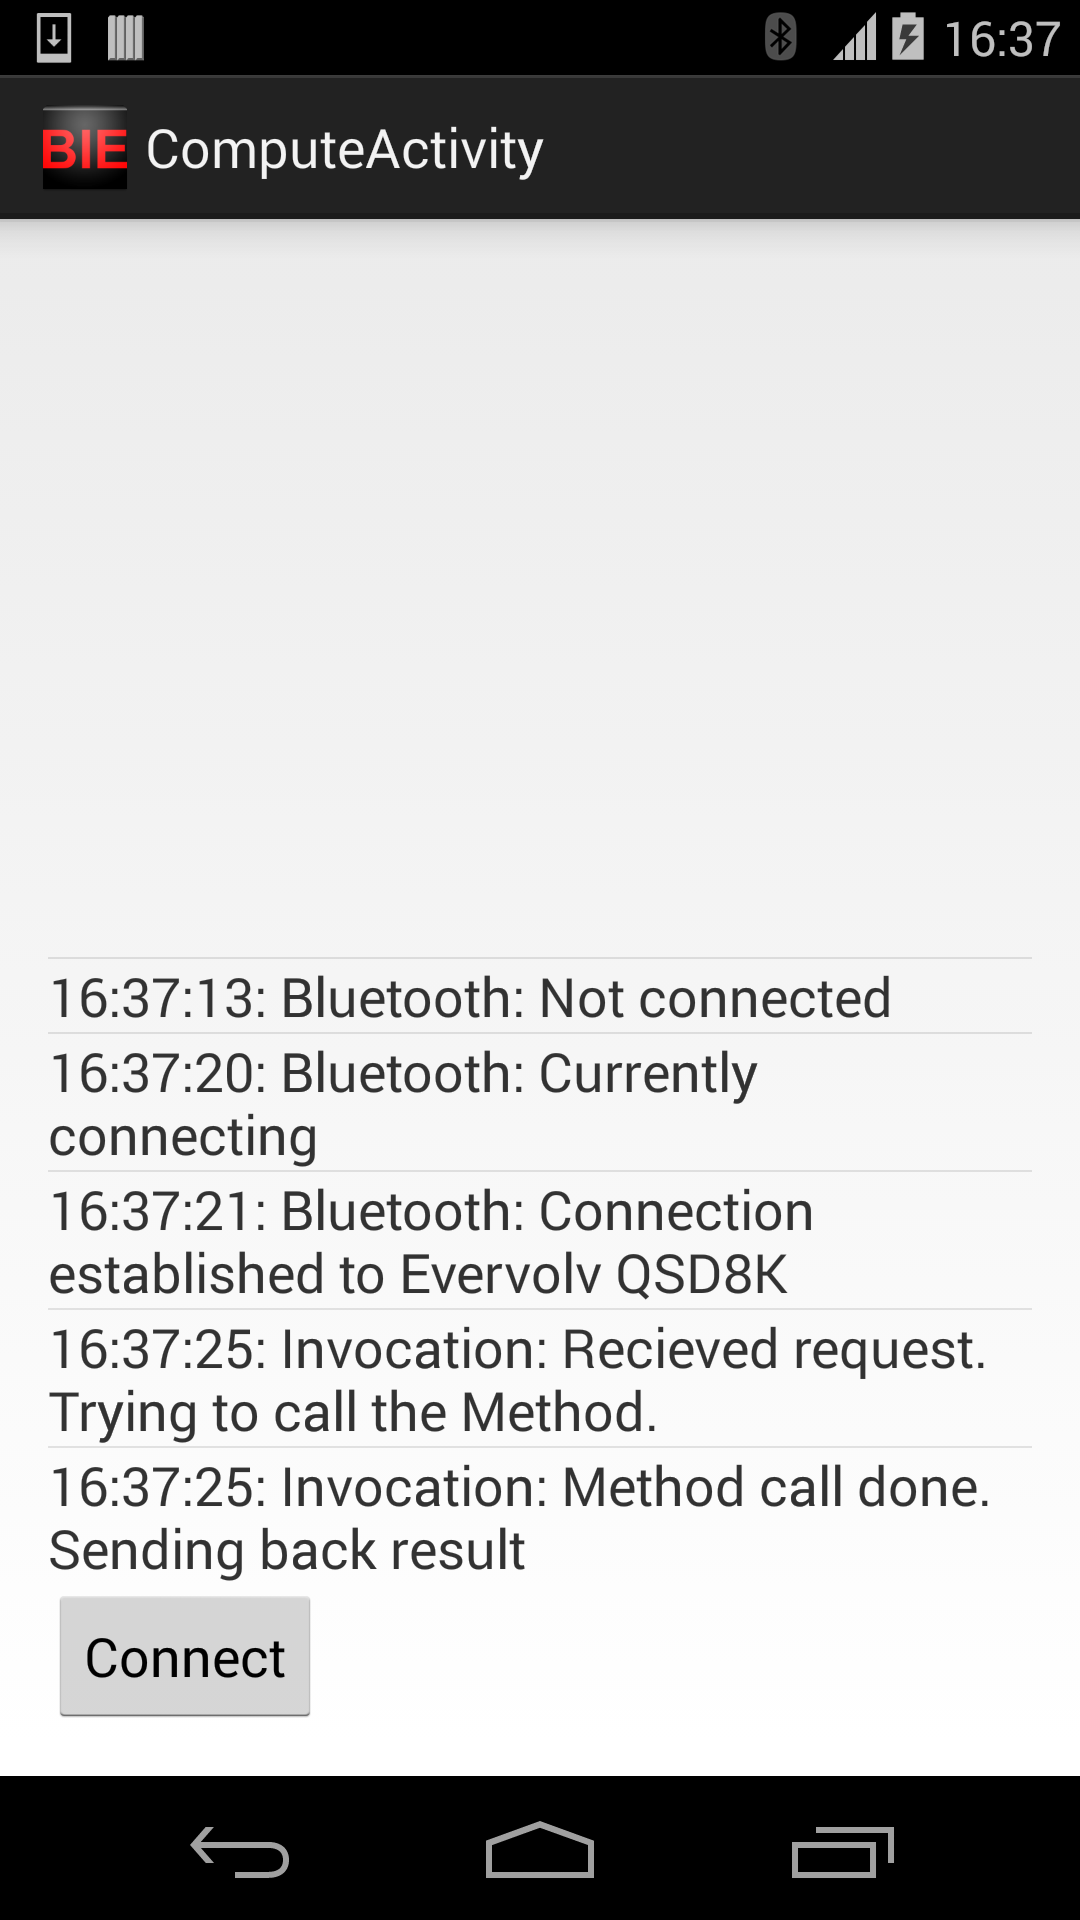
\includegraphics[width=.8\textwidth,keepaspectratio]{ex_compute}
    \captionof{figure}{UI von \lstinline{StartActivity}}
    \label{fig:ex_compute}
\end{minipage}
%
